\documentclass[11pt,landscape,a4paper]{article}
\usepackage[utf8]{inputenc}
\usepackage[ngerman]{babel}
\usepackage[T1]{fontenc}
%\usepackage[LY1,T1]{fontenc}
%\usepackage{frutigernext}
%\usepackage[lf,minionint]{MinionPro}
\usepackage{tikz}
\usetikzlibrary{shapes,positioning,arrows,fit,calc,graphs,graphs.standard}
\usepackage[nosf]{kpfonts}
\usepackage[t1]{sourcesanspro}
\usepackage{multicol}
\usepackage{wrapfig}
\usepackage[top=10mm,bottom=15mm,left=10mm,right=10mm]{geometry}
\usepackage[framemethod=tikz]{mdframed}
\usepackage{microtype}
\usepackage{pdfpages}
\usepackage{amsmath}
\DeclareMathOperator*{\argmax}{\arg\!\max}
\DeclareMathOperator*{\argmin}{\arg\!\min}
\definecolor{myblue}{cmyk}{1,.72,0,.38}

\makeatletter % Author: https://tex.stackexchange.com/questions/218587/how-to-set-one-header-for-each-page-using-multicols
\renewcommand{\section}{\@startsection{section}{1}{0mm}%
                                {.2ex}%
                                {.2ex}%x
                                {\color{myblue}\sffamily\small\bfseries}}
\renewcommand{\subsection}{\@startsection{subsection}{1}{0mm}%
                                {.2ex}%
                                {.2ex}%x
                                {\sffamily\bfseries}}
\begin{document}
\small
\begin{multicols*}{3}
\section{Part 1}
\subsection*{Formulas}
\[\sum_{i=0}^{n-1} ar^i = \frac{a(1-r^n)}{1-r}\]
For given rate $r\%$ over time period $t\in[0, T]$,
with annual period $P$,
discount factor $d_{0,T}$ is given
\[d_{0,T} = \left(1+r\% \times \frac{T}{P}\right)^{-1} < 1\]
\subsection*{No Arbitrage Argument}
To prove $A=B$, show strategies for $A\neq B$.
If $A>B$, short on $A$, long on $B$, and vice versa.
\subsection*{1.1.2 Asset w/ Predictable Income}
\[F_0 = (S_0-C)/d_{0,T}, where C = C'd_{0,t}\]
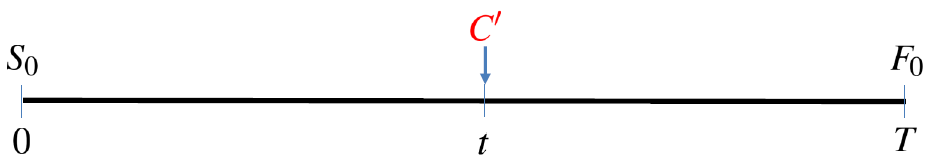
\includegraphics[width=\linewidth]{contents/1.1.2.png}
\subsection*{1.1.3 Asset w/ Continuous Dividend Yield}
Annualized continuous dividend yield of $q$
\[F_0=S_0\exp((r-q)T)\]
\subsection*{1.1.4 Asset w/ Storage Costs}
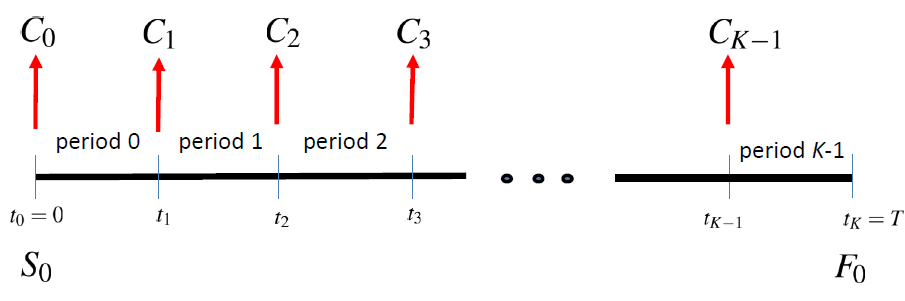
\includegraphics[width=\linewidth]{contents/1.1.4.png}
\[d_{0,K} F_0 = S_0 + \sum_{j=0}^{K-1}d_{0,j}C_j\]
\subsection*{1.1.5 Convenience Yield}
\[d_{0,K} F_0 = S_0 + \sum_{j=0}^{K-1}d_{0,j}(C_j-y)\]
\subsection*{1.2 Value of Forward}
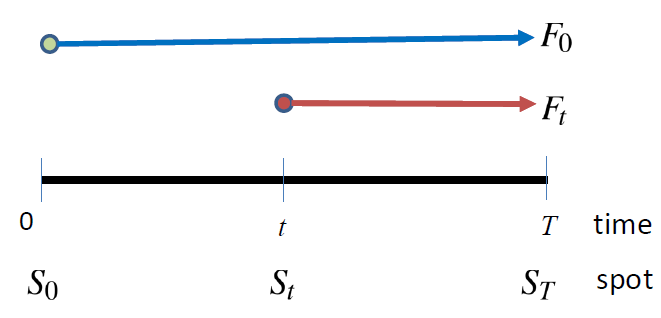
\includegraphics[width=\linewidth]{contents/1.2.png}
\[f_t = (F_t-F_0)d_{t,T}\]

\section{Forwards \& Futures in Practice}
\subsection*{2.1.1 US Treasury Bills}
\begin{itemize}
    \item \textbf{Dollar price}: Typically quoted per \$100 of face value
    \item Often given as \textbf{discount yield} $d$
    \[d=\frac{Par-P}{Par}\times\frac{360}{D}\]
    where $D$ is days to maturity.
    \item Dollar Price is then
    \[P=Par\times\left(1-d\times\frac{D}{360}\right)\]
    \item True yield is the \textbf{coupon equivalent yield} (CEY)
    or \textbf{investment rate}
\end{itemize}
\begin{enumerate}
    \item T-bills not more than half-year to maturity
    \[i=\frac{100-P}{P}\times\frac{y}{t}\]
    \item T-bills more than half-year to maturity. Root of
    \[\left(\frac{t}{2y}-0.25\right)i^2 + \frac{t}{y}i + \frac{P-100}{P}=0\]
\end{enumerate}

\subsection*{2.1.2 Accrued Interest}
\begin{center}
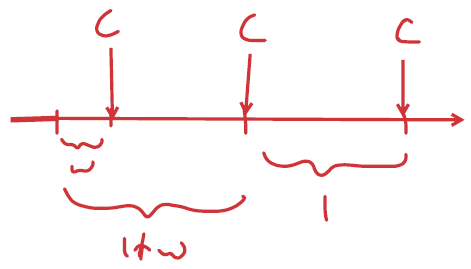
\includegraphics[width=0.3\linewidth]{contents/2.1.2.png}
\end{center}
Bond price a.k.a. \textbf{full, dirty, or invoice price}
\[P = \frac{F}{\left(1+\frac{r}{m}\right)^{w+n-1}}
+\sum_{i=0}^{n-1}\frac{C}{\left(1+\frac{r}{m}\right)^{w+i}}\]
Quoted prices a.k.a. \textbf{clean or flat price} 
does not include accrued interest.
\[DPrice=CPrice+AI\]

\subsection*{2.2.1 Repurchase Agreements}
\begin{itemize}
    \item Repurchase agreements = \textbf{repo} 
    = \textbf{collateralized loan}.
    \item Underlying security held as \textbf{collateral} 
    by counter-party.
    \item Counter-party entered \textbf{reverse repo}.
    \item Rate involved is \textbf{repo rate}.
    \item \textbf{Simple interest} rates. actual/360 in US.
\end{itemize}
\begin{center}
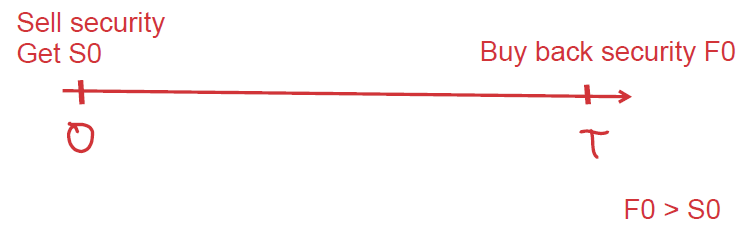
\includegraphics[width=0.5\linewidth]{contents/2.2.1.png}
\end{center}
\begin{enumerate}
    \item At time $t=0$, trader finances purchase of security worth $S_0$.
    \item Enter $T$-day repo with Mr. Y.
    \item Mr. Y demands haircut of $h\%$ and repo rate $r$.
    \item Mr. Y lends $S_0(1-h\%)$.
    \item Trader has net outflow of $S_0\times h\%$.
    \item At time $t=T$, trader pays $F=S_0(1-h\%)(1+r\times T/360)$.
    \item Trader receives security.
    \item Equivalent to forward purchase of security at forward price $F$.
    \item If security price increases to $S_T$ then trader earns profit.
    \item To carry out bet on decline using reverse repo, 
    buy at $S_0$, sell at $S_0(1-h\%)$, buy back at $S_T$.
\end{enumerate}

\subsection*{2.2.2 SOFR}
Secured Overnight Financing Rate (SOFR). Day count: actual/360.
Compound SOFR Formula
\[r=\left[\prod_{i=1}^{T}\left(1+\frac{r_i n_i}{Y}\right)-1\right]\frac{Y}{d_c}\]
Simple SOFR Formula
\[r=\frac{1}{d_c}\sum_{i=1}^T r_i n_i\]

\subsection*{2.2.3 1-Month and 3-Month SOFR Futures}
\begin{itemize}
    \item 1-month SOFR Futures: \$5m loan for 1-month
    \item 3-month SOFR Futures: \$1m loan for 3-months
    \item SOFR Futures follow 30 day periods
    \item Quoted Futures price 1-month: $100\times(1-E(r_m))$, 
    where $r_m$ is the simple average SOFR for contract month
    \item Final Settlement price 1-month: $100\times(1-r_m)$.
    \item Quoted Futures price 3-months: 
    $100\times(1-$ expected compound average SOFR for contract period)
\end{itemize}
\begin{itemize}
    \item Long position gains when expected SOFR falls (futures rises).
    \item Take up long position to hedge against rate falls.
    \item Long position is equivalent to agreeing to lend at rate 
    \[(100-F_0)\%\]
    \item Short position gains when expected SOFR rises (futures falls).
    \item Take up Short position to hedge against rate rises.
    \item Short position is equivalent to agreeing to borrow at rate 
    \[(100-F_0)\%\]
\end{itemize}
Changes to margin account
\begin{itemize}
    \item 1-month: Decrease in futures price by 0.01 (rate rise by 1 bp)
    results in long position being decreased by \$41.67.
    \item 3-months: Decrease in futures price by 0.01 (rate rise by 1 bp)
    results in long position being decreased by \$25.
\end{itemize}
\begin{center}
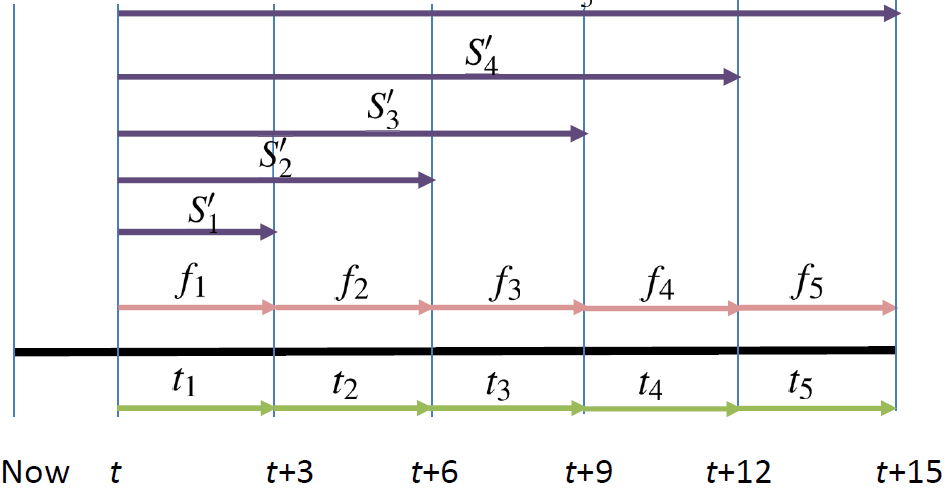
\includegraphics[width=0.6\linewidth]{contents/2.2.3.png}
\end{center}

\subsection*{2.2.4 Treasury Bond Futures}
Hypothetical 30-year 6\% (semi-annual) coupon bond w par value of \$100,000.
\[P_{inv} = N\times F_T \times CF + AI\]
Conversion Factor (CF) is clean price of \$1 coupon bond 
with maturity equal to deliverable bond if priced to yield 6\%.\\
With $n$ remaining coupon payments,
\[P=\frac{1}{1.03^{w+n-1}}+\sum_{i=0}^{n-1} \frac{c}{1.03^{w+i}}-c(1-w)\]
$w\in\{0.5,1\}$ is rounded to nearest quarter.\\
$CPrice$ is quoted bond price. $F_t$ is futures price.

Cheapest-to-Deliver (CTD)\\
$0$ is last coupon date, $t$ is till current date, 
$t+D$ until delivery, $T$ until next coupon
\[DPrice = CPrice + AI_t\]
\[AI_t = \frac{t}{T}\times \frac{c}{2}\times\$100\]
\[AI = \frac{t+D}{T}\times \frac{c}{2}\times\$100\]
Gross Basis
\[GB = CPrice - F_t \times CF\]
Net Basis
\[NB = DPrice \times (1+r\frac{D}{360})-(F_t\times CF + AI)\]
Implied Repo Rate (IRR)\\
rate of return from selling bond futures, then buying actual bond
\[IRR=\frac{(F_t\times CF + AI) - DPrice}{DPrice}\times \frac{360}{D}\]
\begin{center}
    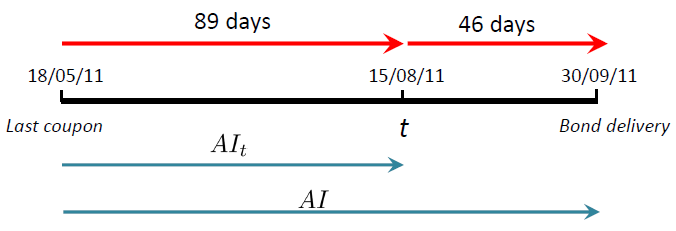
\includegraphics[width=0.6\linewidth]{contents/2.2.4.png}
\end{center}
\[t=89, D=46, T=185\]

\subsection*{2.2.5 Forward Rate Agreements (FRA)}
E.g. FRA covering period one month and ending four months is $1\times4$ contract.
Pricing FRAs, X is fixed rate (actual/360), y is actual ref rate (actual/360).
\[X = \left(\frac{d_{0,T}}{d_{0,T+m}}-1\right)\times\frac{360}{m}\]
Value of FRA
\[v=[d_{t,T} - \left(1+X\times\frac{m}{360}\right)\times d_{t,T+m}]\times N\]

\subsection*{2.3.1 Currency Prepaid Forward}
\[F_0^p=x_0 d_{0,T}(r_u)\]
for interest rate $r_u$, current exchange rate $x_0$.

\subsection*{2.3.2 Currency Forward}
\[F_0 = F_0^p / d_{0,T}(r_s)\]
Essentially the forward exchange rate.

\subsection*{2.3.3 Currency Futures}
FX futures convention: \textbf{base-currency/terms-currency}.
\section{Swaps}
\subsection*{3.2.1 Swap Rate}
\[N-d_{0,K}N=N(1-d_0,K)\]
\[r = \frac{1-d_{0,K}}{\sum_{i=1}^K \frac{t_i}{360}d_{0,i}}\]
\subsection*{3.2.2 Valuation of Swap}
\[B_{fl} = (N+f_1)\exp{-r_1 t_1}\]
\[B_{fix} = N\exp{-r_n t_n} + \sum_{i=1}^n k\exp{-r_i t_i}\]
\[V=B_{fix}-B_{fl}\]

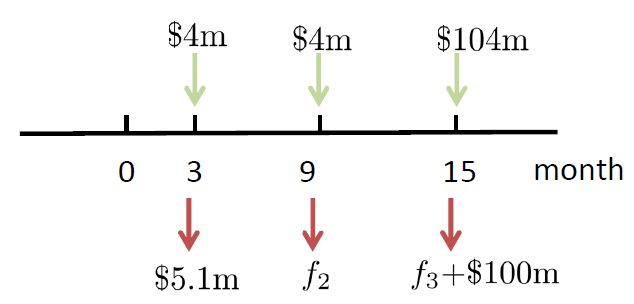
\includegraphics[width=0.3\linewidth]{contents/3.2.2.png}

\subsection*{3.2.3 Arranging a Swap}
A desires floating rate, B wants fixed rate.
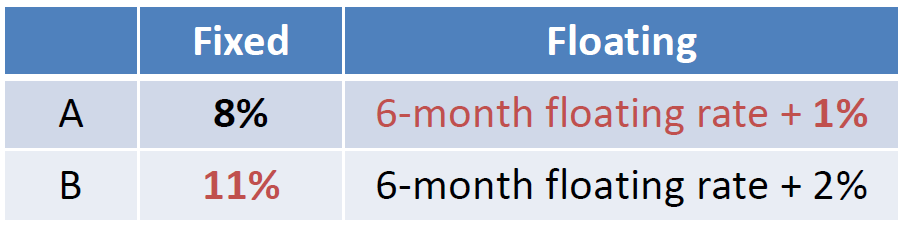
\includegraphics[width=0.3\linewidth]{contents/3.2.3.1.png}
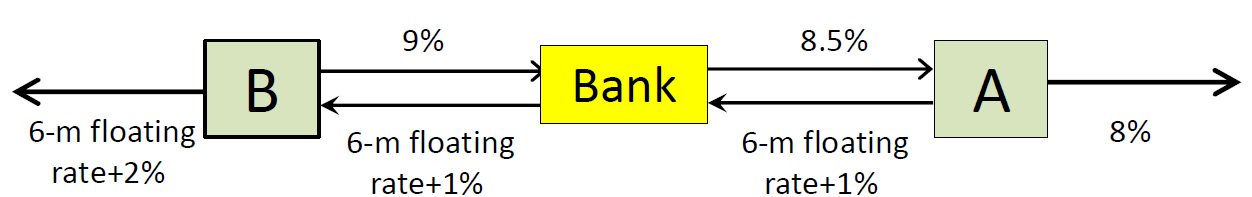
\includegraphics[width=0.3\linewidth]{contents/3.2.3.2.png}
\section{Options}

\subsection*{4.1.1 European Vanilla Options}

Holder of European call, payoff
\[\phi(T) = \max(0,S_T-X)\]
Profit
\[\phi(T) -c/d_{0,T}\]

Holder of European put, payoff
\[\phi(T) = \max(0,X-S_T)\]
Profit
\[\phi(T) -p/d_{0,T}\]

\subsection*{4.2.1 Options and Underliers}
\begin{itemize}
    \item Short Call, Long Asset (Buy-Write) (Covered Call)
    \item Long Put, Long Asset (Protective Put)
\end{itemize}

\subsection*{4.2.2 Spreads}
Assume $X_i < X_j \Leftrightarrow i < j$
\begin{itemize}
    \item Bull Spread - Long Call $X_1$, Short Call $X_2$\\
    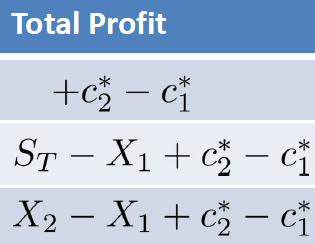
\includegraphics[width=0.2\linewidth]{contents/4.2.2.1.png}
    \item Bear Spread - Short Put $X_1$, Long Put $X_2$\\
    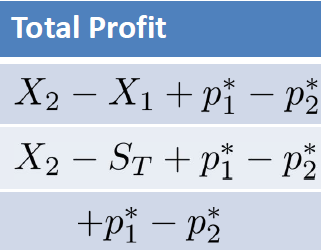
\includegraphics[width=0.2\linewidth]{contents/4.2.2.2.png}
    \item Box Spread - Combine Bull + Bear Spread, $PV=(X_2-X_1)d_{0,T}$
    \item Butterfly Spread - Long Call $X_1,X_3$, Short Call 2x $X_2$, $c_b=c_1+c_3-2c_2$\\
    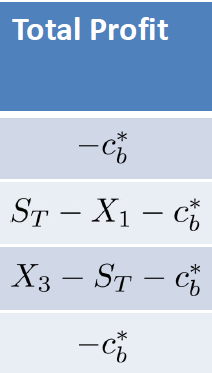
\includegraphics[width=0.1\linewidth]{contents/4.2.2.4.png}
\end{itemize}

\subsection*{4.2.3 Combination}
\begin{itemize}
    \item (Top) Straddle - Long Call, Long Put $X$
    \item Strip - Long Call, Long 2x Put $X$
    \item Strap - Long 2x Call, Long Put $X$
    \item Strangle - Long Call $X_2$, Long Put $X_1$
\end{itemize}
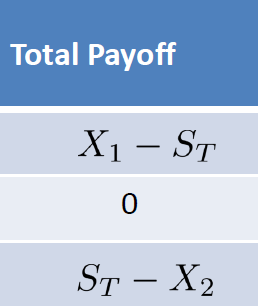
\includegraphics[width=0.1\linewidth]{contents/4.2.3.4.png}

\section{Value at Risk (VaR)}

\subsection*{5.1.1 Definition}
"We are $c\%$ confident (conf. lvl.) that we will not lose 
more than $\$V$ (VaR) in the next $N$ days (risk horizon)."
\[P(L>VaR) \leq 1-c\]
\subsection*{5.1.2 Non-parametric VaR}
Let $V_0,R$ be initial portfolio value and rate of return.
$\mu,\sigma$ are mean and stdev.
\[V=V_0(1+R)\]
Porfolio value $V^*$ at rate of return $R^*$.
\[V^*=V_0(1+R^*)\]
\textbf{Relative VaR}
\[VaR_r = E(V)-V^*=-V_0(R^*-\mu)\]
\textbf{Absolute VaR}
\[VaR_a=V_0-V^*=-V_0R^*\]
Short horizon, $\mu\approx 0, VaR_a\approx VaR_r$.
\[P\&L=V-V_0=\Delta V=V_0R\]
$R$ is \textbf{risk factor}, $V_0$ is \textbf{dollar exposure to $R$}.\\
Given $c$, we find $(1-c)\times$ total obs. to the left,
and interpolate between obs. to get $P\&L^*$.

\subsection*{5.1.3 Parametric VaR}
\[R^* = \mu-\alpha\sigma\]
\[VaR_r = \alpha\sigma\sqrt{\Delta t} V_0\]
\[VaR_a = (\alpha\sigma\sqrt{\Delta t}-\mu)V_0\]
\begin{table}[]
\begin{tabular}{|l|l|l|l|l|l|l|l|}
\hline
Confidence c (\%) & 99.99 & 99.99 & 99    & 97.5  & 95    & 90    & 50 \\ \hline
$\alpha$          & 3.719 & 3.090 & 2.326 & 1.960 & 1.645 & 1.282 & 0  \\ \hline
\end{tabular}
\end{table}
\[N-day VaR=1-day VaR\times\sqrt{N}\]

\subsection*{5.2 Valuation}
\subsection*{5.2.1 Delta-Normal}
\[\Delta V \approx \Delta_0 \Delta S = (\Delta_0 S)\frac{\Delta S}{S}\]
\[VaR=\alpha\sigma|\Delta_0|S_0\]
\[\sigma_p V_t = \sqrt{\sigma_{\Delta v}^2}\]
$\frac{\Delta S}{S}$ is \textbf{risk factor}, 
$\Delta_0 S$ is \textbf{dollar exposure to risk factor}.\\
Duration model
\[\Delta P = -DP\Delta y\]
\[\sigma_P = DP\sigma_y\]

\subsection*{5.3 Delta-Normal Methods}
Exposure vector for weight vector $\mathbf{w_t}$
\[\mathbf{x_t}=[x_{1,t}, x_{2,t}, ..., x_{N,t}]^T=\mathbf{w_t}V_t\]
\[\sigma_{\Delta V}^2 = \sigma_p^2 V_t^2 = \mathbf{x_t^T C_{t+h}x_t}\]
\[VaR_p = \alpha\sqrt{\mathbf{x_t^T C_{t+h}x_t}}\]
\[\mathbf{C}= 
\begin{bmatrix}
    \sigma_1 & \rho\sigma_1 \sigma_2 \\
    \rho\sigma_1 \sigma_2 & \sigma_2 
\end{bmatrix}
\]

\subsection*{5.5 Risk Mapping}
Semiannual bonds.
Standard maturities: 
1,3,6 months, 
1,2,3,4,5,7,9,10,15,20,30 years
\[PV=\frac{x}{(1+y)^t}\]
\[Z_{1.5} = \beta Z_{1.5} + (1-\beta Z_{1.5}) = Z_1 + Z_2\]
\[y_{1.5} = \gamma y_1 + (1-\gamma)y_2\]
\[\sigma_{1.5} = \gamma\sigma_1 + (1-\gamma)\sigma_2\]
$\gamma$ used to interpolate.
\[a\beta^2 + b\beta + c=0\]
\[a=\sigma_1^2 + \sigma_2^2 - 2\rho\sigma_1\sigma_2\]
\[b=2\rho \sigma_1\sigma_2-2\sigma_2^2\]
\[c=\sigma_2^2-\sigma_{1.5}^2\]
\[\mathbf{C} =
\begin{bmatrix}
    \sigma_1 & \dots & 0 \\
    \vdots & \ddots & \vdots \\
    0 & \dots & \sigma_N 
\end{bmatrix}
corr(X)
\begin{bmatrix}
    \sigma_1 & \dots & 0 \\
    \vdots & \ddots & \vdots \\
    0 & \dots & \sigma_N 
\end{bmatrix}
\]
\end{multicols*}
\end{document}